% !TEX root = MutationTestingSurvey.tex

\section{Building Blocks of the Data-driven Automated Test Suites Augmentation Process}
\label{sec:testGenerationData}

The objectives of test suites augmentation have been introduced in Section~\ref{sec:data:test_suite_augmentation}.
In this section, we present solutions that automate two activities required to augment test suites
\emph{Identify Test Inputs} and \emph{Generate Test Oracles}.

\subsection{Automated Identification of Test Inputs}

The goal of the automated identification of test inputs is to generate test inputs that increase the \emph{\% of Operators Applied} when performing data-driven mutation testing. Despite the literature does not address the problem of automatically generating test inputs for data mutation testing, in this section we provide references to related work that can be reused for this purpose. We group the applicable approaches according to the type of models used to drive the mutation testing process: UML models, grammars, block models, no models. 

Automated test inputs generation aims to automatically generate data that can be altered through a mutation operator. 
In the context of system testing, which is the target of data-driven mutation testing, test input data is provided through input interfaces. However, since data-driven mutation testing can be applied to target data exchanged through 
every communication layer, including input interfaces and interfaces used for the communication among internal components, we may observe two possible situations. First, the data exchanged on the communication layer targeted by mutation testing coincide with the input data (i.e., it was not transformed internally). Second, the data exchanged on the communication layer targeted by mutation is the result of a transformation of the input data. For all the approaches targeted in our survey, we thus need to consider both the two cases.

\subsubsection{UML models}
%model-based fuzzying and 

In the case of modelling based on UML models, a data mutation operator may not be applied during mutation testing when the type of data that it is supposed to alter is not observed during the execution of the test cases. 
For example, in the case of the data model in Figure~\ref{fig:dataModel}, we may not be able to apply the operator \emph{Attribute Replacement with Random} to the attribute \emph{destinationId} of class \emph{GpsrPacketHeader} if all the test cases contain messages with \emph{SarPacketHeaders}.



When the data exchanged on the communication layer targeted by mutation testing coincide with the input data, existing approaches based on constraint-solvers can be adopted. 
These approaches rely on a formal or semi-formal specification of the structure of the input data and the constraints among data fields.
Some techniques target the generation of inputs whose data structure had been specified using a UML class diagram where the relations among data fields have been captured using OCL constraints. The data structure model is a UML class diagram and resemble the one reported in Figure~\ref{fig:dataModel}. The OCL language is instead used to capture all the constraints among data fields. Existing techniques in this category work by generating class diagram instances that satisfy a set of given OCL constraints by executing appropriate constraint solvers after having transformed the OCL constraints into other formalisms such as Alloy models~\cite{Uml2alloy}, constraint satisfaction~\cite{EMFTOCSP}, SMT~\cite{Przigoda2016}, or SAT problems~\cite{Soeken2011}. 

Other approaches, instead, work with models specified in formats other than UML class diagrams:
Java classes~\cite{Boyapati-KORAT-ISSTA-2002,gligoric2010test}, constraint logic~\cite{Senni-CPLgeneration-TAP-2012}, Alloy~\cite{Khurshid-SpecificationBasedTesting-ASE-2004}, or Z specifications~\cite{Horcher-Z-1995}.
These techniques have been proven to be effective for testing software systems that process classical data structures like trees. 
Alloy is a modelling language for expressing complex structural constraints~\cite{Jackson:Alloy:2002},
which has been successfully used to generate test inputs for testing object-oriented programs~\cite{Khurshid-SpecificationBasedTesting-ASE-2004}.
Korat, instead, is a technique that allows to generate data structures to test Java programs~\cite{Boyapati-KORAT-ISSTA-2002}. Given a bound to the input structures, i.e. the maximum number of instances for each class to be used, Korat exhaustively generates all the nonisomorphic structures that are valid. 
Some of the limitations of Korat include requiring the definition of an imperative predicate that evaluates the correctness of the generated structure, which could be complex in the case of complex data models, requiring the manual definition of an input bound for each non primitive attribute or association, which might be particularly expensive in case of complex data structure,  not dealing with constraints defined over integers.
A more efficient, black-box test generation approach is UDITA~\cite{gligoric2010test}.
What contributes to the efficiency of UDITA is the combination of both generator methods and predicates.
Generator methods are used to build instances of the data structure, while predicates are used to validate the generated instances. UDITA relies upon the Java Path Finder model checker~\cite{Visser-JPF-2004} to generate all the instances that satisfy the given predicates. However, the implementation of these generator methods that define the complete structure of a complex data model instance and lead to realistic test inputs can be quite expensive. 

A common limitation of solutions based on constraint-solvers is their scalability~\cite{di2017augmenting}. In the context of mutation testing, where existing test inputs are available, a possible solution to address the scalability problem may consist of generating new test inputs by regenerating only portions of existing test inputs.
For example, Di Nardo et al.~\cite{di2017augmenting} automatically generate test inputs for new requirements by adapting existing field data.
This is achieved by combining model transformations with constraint solving as shown in Fig.~\ref{fig:DiNardo}.
Model transformations enable the partial reuse of existing field data, while constraint solving allows for the generation of missing data. The approach requires a model of the structure of the data provided by using an UML class diagram with OCL expressions capturing the constraints among data fields. In the case of Di Nardo et al., the missing data corresponds to new data types and constraints introduced after updating the requirements of the software under test. In the context of mutation testing, these may correspond to data types not observed during the execution of the test suite.
In Step 1, a chunk of data is loaded in memory as an instance of the original data model (Original Model Instance).
A dedicated parser is used for that purpose.
In Step 2, a model transformation applied to the Original Model Instance is used to generate an instance of the Updated Data Model. The result is an instance of the Updated Data Model that is incomplete (Incomplete Model Instance).
It contains only the information that can be directly derived from the Original Model Instance:
instances of classes and attributes that have been introduced in the Updated Data Model are missing from the Incomplete Model Instance (these instances are the ones generated in the next steps of the algorithm).
In Step 3, UML2Alloy~\cite{Uml2alloy} is used to generate an Alloy model that corresponds to the class diagram and the OCL constraints of the data model; the Alloy Analyzer~\cite{AlloyWeb} is then used to generate  valid instances of the updated data model by means of constraint solving. 
Finally, in Step 4, to generate the concrete test inputs to be processed by the software under test (e.g. a binary file), the content of the Valid Model Instance is written in the format processed by the software under test through a dedicated encoder.
Despite empirical results show a huge performance gain with respect to traditional constraint-based approaches, the need for dedicated parsers to translate existing test inputs into class diagram instances may limit the applicability of the approach. Also, the available test inputs may not enable the generation of all the inputs data needed.

\begin{figure}[t!]
  \centering
    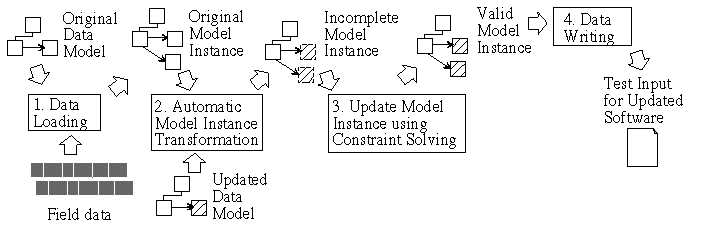
\includegraphics{images/DiNardoTOSEM}
      \caption{Automatic generation of test inputs for new data requirements proposed by Di Nardo et al~\cite{di2017augmenting}.}
      \label{fig:DiNardo}
\end{figure}

Other approaches address the scalability problem by relying on hybrid approaches~\cite{soltana2019practical}.
For example, PLEDGE~\cite{soltana2019practical} combines metaheuristic search and Satisfiability Modulo Theories (SMT~\cite{SMT:2011}) to generate UML instance models from UML class diagrams annotated with OCL constraints. It  works by using the Negation Normal Form (NNF~\cite{NNF:2001}) to represent all the constraints derived from the UML data model. Different subformulas that build the NNF formula are then solved by combining metaheuristic search and SMT. Metaheuristic search is used to handle subformulas whose satisfaction involves structural tweaks to the instance model, i.e., additions and deletions of objects and links. SMT is used with subformulas involving only primitive attributes, i.e., attributes with primitive types. 


When the data exchanged on the communication layer targeted by mutation is the result of a transformation of the input data, the only applicable solution consist in the application of approaches that generate inputs from scratch. By generating a large number of inputs that include instances for all the classes of the data model, these approaches may, in principle, lead to the generation of required data by internal components. However, without means to drive the generation of such data, the application of UML-based test input generation approaches in these situation is likely to be inefficient.

%Despite this approach enables efficient generation of test inputs from scratch, it may still require dedicated parsers for the con

\subsubsection{Grammars}

When grammars are used to model the input, traditional grammar-based test input generation approaches relying on the expansion of the production rules of the grammar can be adopted~\cite{fuzzingbook2019:GrammarFuzzer}. 
Available tools are shown in Table~\ref{table:grammarGeneration}.

\begin{table}[h]
\caption{List of tools for grammar-based inputs generation.}
\label{table:grammarGeneration}
\begin{center}
\tiny
\begin{tabular}{|p{2cm}|p{2cm}|p{2cm}|p{7cm}|}
\hline
\textbf{Name}&\textbf{Grammar}&\textbf{Licence}&\textbf{Description}\\
\hline
GramTest~\cite{GramTest}& BNF&Apache 2.0&Java-based tool that allows you to generate test cases based on BNF grammars. It covers all the production rules of the grammar.\\
\hline
Fuzzingbook Grammar Coverage-based Fuzzer~\cite{fuzzingbook2019:GrammarFuzzer}& BNF & MIT &Python tool that implements production rules coverage. It implements the Shortest Path Selection~\cite{Burkhardt:TestFromSyntax} optimization.\\
\hline
GP~\cite{GPlib,Kifetew:GBTest:2017}& Annotated BNF & Proprietary& Tool for the automated generation of inputs from Stochastic Context Free Grammars. Implemented on top of genetic programming algorithms. https://selab.fbk.eu/kifetew/downloads/gplib-607.jar\\
RIDDLE~\cite{ghosh1998testing}&BNF& Proprietary& Tool that adopts a grammar to describe the format of inputs; based on the grammar, random and boundary values are generated for tokens representing input parameters.\\
\hline
\end{tabular}
\end{center}
\end{table}%

Similarly to the case of UML-based test case generation approaches that generate inputs from scratch, these grammar-based approaches can be adopted when the communication layer targeted by mutation testing is either the input layer or an internal layer.However, they may suffer of inefficiency problems.

%\cite{grammar:survey}

\subsubsection{Block-models}

TO BE COMPLETED

\TODO{Fabrizio}

\subsubsection{No models}


TO BE COMPLETED
\TODO{Fabrizio}

\endinput

